\documentclass{article}
\usepackage{hyperref}
\hypersetup{colorlinks=true,urlcolor=blue}
\usepackage{listings}
\usepackage{geometry}
\geometry{margin=1in}
\usepackage{graphicx}
\graphicspath{ {./hw2/} }
\begin{document}
\title{BMI 203: Algorithms - Homework 2}
\author{Laurel Estes}
\maketitle
\section{Implementing Hierarchical and Parition-Based Clustering}
\subsection{Similarity Metric}
Given the limited scope of the project, I chose to implement a very basic (and to a large extent arbitrary) similarity metric, which is to calculate a linear combination of the following: length of the active site (in number of residues), surface area-to-volume ratio of the active site in space, and (given two sites for which similarity is being measured) the euclidean distance between the 6-element vectors formed by the percentages of residues in each site belonging to each of 6 physiochemical categories of amino acid (nonpolar, cysteine, polar uncharged, positive, negative, and bent). Active sites of enzymes rely on their physical shape and their local chemistry in order to catalyze reactions, and I wanted my metric to attempt to get at these properties without relying on amino acid sequence. My reasoning was that (for this project) I am most interested in trying to cluster sites that bind similar ligands, and for this purpose, the amino acid chemistry is more important than the amino acid identity, unlike in a DNA sequence. Furthermore, residues in sites are not necessarily a single continuous part of the protein, the residues are not necessarily arranged such that a linear sequence of residues maps well onto the structure for purposes of understanding local chemistry information. \par
Given more time, I would have liked to try to compare overall shape/size by overlaying the boxes formed by the active site dimensions, and potentially integrate some component of amino acid sequence data to try and capture information about what residues are next to each other (are there patches of polar vs nonpolar, etc.) I spent some time reading up on the PARIS algorithm (Hoffmann et al., 2010) and liked their general methodology of combining volumetric measurements with alignments of "probability clouds" of physical structure in order to try and cluster active sites based on similarity of the ligands that they bind. 
\subsection{Hierarchical Algorithm}
\subsection{Partioning Algorithm}
\subsection{Quality Measurement}
\subsection{Comparing Clusterings}
\subsection{Biological Relevance}


%\begin{figure}[h]
%\centering
%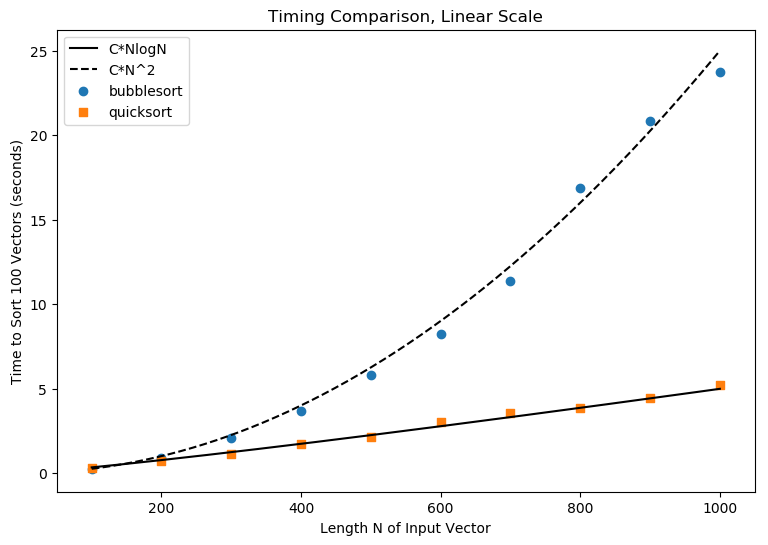
\includegraphics[width=0.6\textwidth]{hw1/fig3.png}
%\end{figure}

\section{Github Repository}
All of the code used in this assignment is on Github: \url{https://github.com/laueste/algorithms-ucsf-2019}
\end{document}